\begin{frame}
  \frametitle{Initializing CMD/RPMD}

  \begin{itemize}
  \item CMD and RPMD are intended to provide approximations to quantum dynamics
    and not to efficiently sample the quantum phase space.
    
  \item The ergodicity problem can be circumvented by launching trajectories
    from many different choice of configurations and momenta.

  \smallskip
  \begin{center}
    \resizebox{0.8\textwidth}{!}
    {
    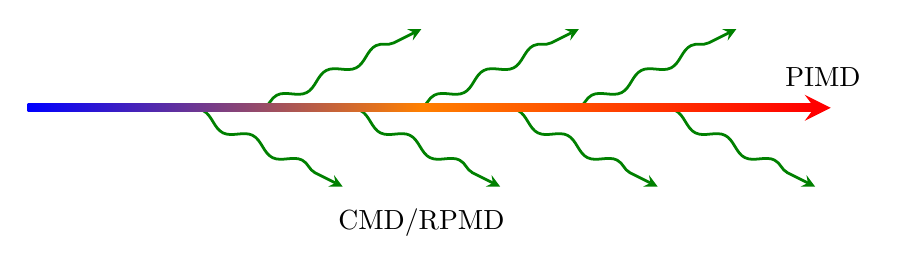
\begin{tikzpicture}

    %   \begin{axis}
    %     [
    %     % axis lines=none,
    %     % enlargelimits=false,
    %     width=0.8\textwidth,
    %     height=0.2\textwidth,
    %     ]
    %     \addplot [
    %         samples=1000,
    %         domain=0:10,
    %         mesh,                   % Use line segments instead of one unbroken line
    %         colormap={}{            % Define the colormap
    %             color(0.0)=(blue);
    %             color(0.2)=(green);
    %             color(1.0)=(red);
    %         },
    %         line width=2pt,
    %         point meta=x            % Define the value that's used to determine the color
    %     ] {0};
    %     \draw[->, >=stealth, line width=2pt, color=red] (10.0, 0.0) -- node
    %     [above, color=black] {PIMD} ++(0.20, 0);
    % \end{axis}
    
    \foreach \x [count=\ii] in {
      2,3,...,8
    }
    {
      % \pgfmathparse{\ii * 5}\edef\y{\pgfmathresult}
      \pgfmathtruncatemacro\y{1.0 * (-1)^\ii}
      \draw[
        line width=1.0pt, ->, >=stealth,
        decorate,
        color=green!50!black,
        decoration={
          snake, amplitude=2.0,
          segment length=20,
          post length=1mm,
        }
      % ] (\x, 0.0) -- ++(0.0, -2.0);
      ] (\x, 1.5pt) -- ++(2.0, \y);
    }
    \shade[left color=blue, right color=red, middle color=orange] (0.0, 0.0) rectangle (10.0, 3pt);
    \draw[->, >=stealth, line width=3pt, color=red, anchor=west]
        (10.0, 1.5pt) -- node [above=3pt, color=black]
        {PIMD} ++(0.20, 0);
    \node[below] at (5.0, -1.1) {CMD/RPMD};
    \end{tikzpicture}
    }
  \end{center}

  \begin{enumerate}
    \setlength{\itemsep}{6pt}%
    \item Run a PIMD trajectory using an efficient thermostat scheme.
    \item Pick configurations and momenta from the thermostatted trajectory and
      launch RPMD or CMD trajectories from them.
    \item Ideally the separation in time between each should be determined by
      the correlation time of the properties in the system.
  \end{enumerate}
  \end{itemize}
 
\end{frame}
